\documentclass[a4paper, 12pt]{article}
\usepackage[utf8x]{inputenc}
\usepackage{cmap}
\usepackage[english, russian]{babel}
\usepackage{indentfirst}
\usepackage[left=20mm, top=20mm, right=20mm, bottom=20mm]{geometry}
\usepackage{tikz}
\usepackage{float}
\usepackage{amsmath, amsfonts, amssymb}
\usepackage{graphicx}
\usepackage{fancybox, fancyhdr}
\usepackage{hyperref}
\usepackage{listings}
\usepackage{caption}
\usepackage{subcaption}
\usepackage{xcolor}
\usepackage{attachfile2}
\pagestyle{fancy}
\fancyhf{}
\fancyhead[L]{Лабораторная работа №2}
\fancyhead[R]{Математическая статистика}
\fancyfoot[C]{\thepage}
\graphicspath{{images/}}
\usetikzlibrary{patterns}
\definecolor{LightGray}{gray}{0.95}
\definecolor{LightGray2}{gray}{0.7}
\lstdefinestyle{code}{
    language=Python, % replace with needed language
    basicstyle=\footnotesize\ttfamily,
    backgroundcolor=\color{LightGray},
    showspaces=false,
    showstringspaces=false,
    showtabs=false,
    tabsize=4,
    captionpos=b,
    breaklines=true,
    breakatwhitespace=false,
    frame=single,
    rulecolor=\color{LightGray2},
    linewidth=\linewidth,
    keywordstyle=\color{blue}\bfseries,
    commentstyle=\color{green!40!black},
    stringstyle=\color{purple},
    escapeinside={\%*}{*)},
    inputencoding=utf8x,
    xleftmargin=0pt,
    framexleftmargin=0pt,
    framexrightmargin=0pt
}
\lstset{style=code}
\hypersetup{
    colorlinks=true,
    linkcolor=blue,
    filecolor=magenta,
    urlcolor=cyan,
    pdftitle={contents setup},
    pdfpagemode=FullScreen,
}
\setlength{\parskip}{1.5mm}
\setlength{\headheight}{15pt}
\setlength{\footskip}{15pt}
\allowdisplaybreaks
\DeclareMathOperator{\sinc}{sinc}
\newcommand{\frc}[2]{\raisebox{2pt}{$#1$}\big/\raisebox{-3pt}{$#2$}}

\begin{document}
    \begin{titlepage}

        \begin{center}
        
\includegraphics[width=0.3\textwidth]{itmo.png} % requires itmo.png in /images folder
        \vfill
        
        Федеральное государственное автономное образовательное учреждение высшего образования
        «Национальный Исследовательский Университет ИТМО»\\
        
        \vfill
        {\large\bf ЛАБОРАТОРНАЯ РАБОТА №2}\\
        {\large\bf ПРЕДМЕТ «МАТЕМАТИЧЕСКАЯ СТАТИСТИКА»}\\
        {\large\bf ТЕМА «ДОВЕРИТЕЛЬНЫЕ ИНТЕРВАЛЫ»}\\
        Вариант 1, 1
        \vfill

        \begin{flushright}
            \begin{minipage}{.45\textwidth}
            {
                \hbox{Преподаватель: Лимар И. А.}
                \hbox{Студент: Румянцев А. А.}
                \hbox{Поток: Мат Стат 31.2}
                \hbox{}
                \hbox{Факультет: СУиР}
                \hbox{Группа: R3341}
            }
            \end{minipage}
        \end{flushright}
        
        \vfill
                
        Санкт-Петербург\\
        2024
        \end{center}
    \end{titlepage}
    
    \tableofcontents

    \newpage
    \section{Задание 1}
    \subsection{Условие}
    Предъявите доверительный интервал уровня $1-\alpha$ для указанного параметра при данных
    предположениях (с математическими обоснованиями). Сгенерируйте 2 выборки объёма объёма
    25 и посчитайте доверительный интервал. Повторить 1000 раз. Посчитайте, сколько раз 
    95-процентный доверительный интервал покрывает реальное значение параметра. То же самое
    сделайте для объема выборки 10000. Как изменился результат? Как объяснить? Что изменяется
    при росте объемов выборок?


    Даны две независимые выборки $X_1$, $X_2$ из нормальных распределений $\mathcal{N}\left(\mu_1,\sigma_1^2\right)$,\\
    $\mathcal{N}(\mu_2,\sigma_2^2)$ объемов $n_1$, $n_2$ соответственно.
    Сначала указывается оцениваемая функция, потом данные об остальных параметрах, затем параметры эксперимента и подсказки.
    $$\tau=\mu_1-\mu_2;\,\sigma_1^2,\,\sigma_2^2\text{ известны};\,\mu_1=2,\,\mu_2=1,\,\sigma_1^2=1,\,\sigma_2^2=0.5;\text{ воспользуйтесь функцией}$$
    $$\dfrac{\overline{X_1}-\overline{X_2}-\tau}{\sigma},\,\,\,\,\sigma^2=\dfrac{\sigma_1^2}{n_1}+\dfrac{\sigma_2^2}{n_2}$$


    \subsection{Выполнение}
    $$Z=\sqrt{n}\cdot\dfrac{\overline{X}-\mu}{\sigma}\sim\mathcal{N}\left(0,1\right)$$
    $$\gamma=1-\alpha$$
    \begin{figure}[H]
        \centering
        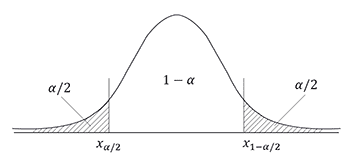
\includegraphics[scale=1.2]{normal.png}
        \captionsetup{skip=0pt}
        \caption{Двусторонняя критическая область}
        \label{fig:normal}
    \end{figure}
    $$r_1=x_{\frac{\alpha}{2}},\,\,r_2=x_{1-\frac{\alpha}{2}}$$
    $$\mathbb{P}\left(r_1\leq\sqrt{n}\cdot\dfrac{\overline{X}-\mu}{\sigma}\leq r_2\right)=\gamma=1-\alpha$$
    $$r_1=-r_2=-x_{1-\frac{\alpha}{2}}$$
    $$\Bigg|\sqrt{n}\cdot\dfrac{\overline{X}-\mu}{\sigma}\Bigg|\leq x_{1-\frac{\alpha}{2}}$$
    $$\overline{X_1}\sim\mathcal{N}\left(\mu_1,\dfrac{\sigma_1^2}{n_1}\right),\,\,\,\,\overline{X_2}\sim\mathcal{N}\left(\mu_2,\dfrac{\sigma_2^2}{n_2}\right)$$
    $$\overline{X_1}-\overline{X_2}\sim\mathcal{N}\left(\mu_1-\mu_2,\dfrac{\sigma_1^2}{n_1}+\dfrac{\sigma_2^2}{n_2}\right)\equiv\overline{X_1}-\overline{X_2}\sim\mathcal{N}\left(\tau,\sigma^2\right)$$
    $$\overline{X_1}-\overline{X_2}-\tau\sim\mathcal{N}\left(0,\sigma^2\right)$$
    $$\dfrac{\overline{X_1}-\overline{X_2}-\tau}{\sigma}\sim\mathcal{N}\left(0,1\right)$$
    $$\sigma=\sqrt{\dfrac{\sigma_1^2}{n_1}+\dfrac{\sigma_2^2}{n_2}}=\sqrt{\dfrac{n_2\cdot\sigma_1^2+n_1\cdot\sigma_2^2}{n_1\cdot n_2}}=\dfrac{\sqrt{n_2\cdot\sigma_1^2+n_1\cdot\sigma_2^2}}{\sqrt{n_1\cdot n_2}}$$
    $$\dfrac{\overline{X_1}-\overline{X_2}-\tau}{\dfrac{\sqrt{n_2\cdot\sigma_1^2+n_1\cdot\sigma_2^2}}{\sqrt{n_1\cdot n_2}}}=\sqrt{n_1\cdot n_2}\cdot\dfrac{\overline{X_1}-\overline{X_2}-\tau}{\sqrt{n_2\cdot\sigma_1^2+n_1\cdot\sigma_2^2}}$$
    $$\Bigg|\sqrt{n_1\cdot n_2}\cdot\dfrac{\overline{X_1}-\overline{X_2}-\tau}{\sqrt{n_2\cdot\sigma_1^2+n_1\cdot\sigma_2^2}}\Bigg|\leq x_{1-\frac{\alpha}{2}}\Rightarrow
    \Bigg|\overline{X_1}-\overline{X_2}-\tau\Bigg|\leq x_{1-\frac{\alpha}{2}}\cdot\dfrac{\sqrt{n_2\cdot\sigma_1^2+n_1\cdot\sigma_2^2}}{\sqrt{n_1\cdot n_2}}$$
    $$-x_{1-\frac{\alpha}{2}}\cdot\dfrac{\sqrt{n_2\cdot\sigma_1^2+n_1\cdot\sigma_2^2}}{\sqrt{n_1\cdot n_2}}\leq\overline{X_1}-\overline{X_2}-\tau\leq x_{1-\frac{\alpha}{2}}\cdot\dfrac{\sqrt{n_2\cdot\sigma_1^2+n_1\cdot\sigma_2^2}}{\sqrt{n_1\cdot n_2}}$$
    $$-\left(\overline{X_1}-\overline{X_2}\right)-x_{1-\frac{\alpha}{2}}\cdot\dfrac{\sqrt{n_2\cdot\sigma_1^2+n_1\cdot\sigma_2^2}}{\sqrt{n_1\cdot n_2}}\leq-\tau\leq -\left(\overline{X_1}-\overline{X_2}\right)+x_{1-\frac{\alpha}{2}}\cdot\dfrac{\sqrt{n_2\cdot\sigma_1^2+n_1\cdot\sigma_2^2}}{\sqrt{n_1\cdot n_2}}$$
    $$\left(\overline{X_1}-\overline{X_2}\right)-x_{1-\frac{\alpha}{2}}\cdot\dfrac{\sqrt{n_2\cdot\sigma_1^2+n_1\cdot\sigma_2^2}}{\sqrt{n_1\cdot n_2}}\leq\tau\leq \left(\overline{X_1}-\overline{X_2}\right)+x_{1-\frac{\alpha}{2}}\cdot\dfrac{\sqrt{n_2\cdot\sigma_1^2+n_1\cdot\sigma_2^2}}{\sqrt{n_1\cdot n_2}}$$
    $$\left(\overline{X_1}-\overline{X_2}\right)-x_{1-\frac{\alpha}{2}}\cdot\sigma\leq\tau\leq \left(\overline{X_1}-\overline{X_2}\right)+x_{1-\frac{\alpha}{2}}\cdot\sigma$$


    \begin{lstlisting}[label=imps1, caption={import}]
    import numpy as np
    import scipy.stats as st
    \end{lstlisting}


    \begin{lstlisting}[label=vars, caption={Задаем данные по условию}]
    mu_1, mu_2 = 2, 1
    tau = mu_1 - mu_2
    sigma2_1, sigma2_2 = 1, 0.5
    n_1, n_2 = 25, 25
    alpha = 0.05
    n = 1
    \end{lstlisting}


    \begin{lstlisting}[label=code1, caption={Код для подсчета доверительного интервала и кол-во попаданий}]
    count = 0
    for i in range(n):
        X_1 = np.random.normal(mu_1, sigma2_1, n_1)
        X_2 = np.random.normal(mu_2, sigma2_2, n_2)
        
        X_1_mean = np.mean(X_1)
        X_2_mean = np.mean(X_2)
        
        sigma = np.sqrt(sigma2_1 / n_1 + sigma2_2 / n_2)
        
        z = st.norm.ppf(1 - alpha / 2)
        
        lower_bound = (X_1_mean - X_2_mean) - z * sigma
        upper_bound = (X_1_mean - X_2_mean) + z * sigma

        print(f'{lower_bound:.4f}<={tau}<={upper_bound:.4f}')
            
        if lower_bound <= tau <= upper_bound:
            count += 1
        
    print(f'covers_tau_count={count}, ratio={count / n}')
    \end{lstlisting}


    \begin{lstlisting}[label=res1, caption={Посчитанный доверительный интервал}]
    0.5934<=1<=1.5536
    \end{lstlisting}


    \begin{lstlisting}[label=res1000cov, caption={Покрывает 95-\% для $n=1000$}]
    covers_tau_count=975, ratio=0.975
    \end{lstlisting}


    \begin{lstlisting}[label=res10000cov, caption={Покрывает 95-\% для $n=10000$}]
    covers_tau_count=9688, ratio=0.9688
    \end{lstlisting}


    Тут будет вывод (очевидно, что точность увеличивается)


    \section{Задание 2}
    \subsection{Условие}
    Постройте асимптотический доверительный интервал уровня $1-\alpha$ для указанного параметра.
    Проведите эксперимент по схеме, аналогичной первой задаче.
    
    
    Сначала указывается класс распределений (однопараметрический),
    затем параметры эксперимента и подсказки.
    $$\text{Ехр}(\lambda);\text{ медиана};\,\lambda=1$$


    \subsection{Выполнение}
    $$f_X(x)=
    \begin{cases}
        \lambda\cdot\exp{\left\{-\lambda x\right\}},& x\geq0\\
        0,& x < 0
    \end{cases}$$


    $$\hat{\theta}_n\xrightarrow{n\to\infty}\mathcal{N}\left(\theta;\dfrac{\sigma^2\left(\theta\right)}{\sqrt{n}}\right)$$
    $$\Bigg|\sqrt{n}\cdot\dfrac{\hat{\theta}_n-\theta}{\sigma\left(\theta\right)}\Bigg|\sim\mathcal{N}\left(0,1\right),\,\,\,\, \Bigg|\sqrt{n}\cdot\dfrac{\hat{\theta}_n-\theta}{\sigma\left(\theta\right)}\Bigg|\leq u_{1-\frac{\alpha}{2}}$$
    $$\hat{\theta}_n-\dfrac{\sigma\left(\theta\right)}{\sqrt{n}}u_{1-\frac{\alpha}{2}}\leq\theta\leq\hat{\theta}_n+\dfrac{\sigma\left(\theta\right)}{\sqrt{n}}u_{1-\frac{\alpha}{2}}$$
    $$\hat{\theta}_n-SE\left[\hat{\theta}_n\right]u_{1-\frac{\alpha}{2}}\leq\theta\leq\hat{\theta}_n+SE\left[\hat{\theta}_n\right]u_{1-\frac{\alpha}{2}}$$
    $$SE\left[\hat{\theta}_n\right]=\sqrt{\text{Var}\left[\hat{\theta}_n\right]}$$
    $$\hat{m}-SE\left[\hat{m}\right]u_{1-\frac{\alpha}{2}}\leq m\leq\hat{m}+SE\left[\hat{m}\right]u_{1-\frac{\alpha}{2}}$$
    $$L\left(\lambda,x\right)=\prod_{i=1}^{n}f_X\left(x\right)=\lambda^n\cdot\exp{\left\{-\lambda\sum\limits_{i=1}^{n}x_i\right\}}$$
    $$\ln{L\left(\lambda,x\right)}=\ln{\left(\lambda^n\cdot\exp{\left\{-\lambda\sum\limits_{i=1}^{n}x_i\right\}}\right)}=
    \ln{\lambda^n}+\ln{\exp{\left\{-\lambda\sum\limits_{i=1}^{n}x_i\right\}}},$$
    $$\ln{\lambda^n}=n\cdot\ln{\lambda},\,\,\,\,\ln{\exp{\left\{-\lambda\sum\limits_{i=1}^{n}x_i\right\}}}=-\lambda\sum\limits_{i=1}^{n}x_i\cdot\ln{e}=-\lambda\sum\limits_{i=1}^{n}x_i,$$
    $$\ln{L\left(\lambda,x\right)}=n\ln{\lambda}-\lambda\sum\limits_{i=1}^{n}x_i$$
    $$\hat{\lambda}=\text{argmax}\left(L\left(\lambda,x\right)\right)\Rightarrow \dfrac{\partial\ln{L\left(\lambda,x\right)}}{\partial\lambda}=0,$$
    $$\dfrac{\partial\ln{L\left(\lambda,x\right)}}{\partial\lambda}=\left(n\ln{\lambda}-\lambda\sum\limits_{i=1}^{n}x_i\right)_{\lambda}^{\prime}=
    \dfrac{n}{\lambda}-\sum\limits_{i=1}^{n}x_i=0\Rightarrow\dfrac{n}{\lambda}=\sum\limits_{i=1}^{n}x_i\Rightarrow\hat{\lambda}=\dfrac{n}{\sum_{i=1}^{n}x_i},$$
    $$\overline{X}=\dfrac{1}{n}\sum\limits_{i=1}^{n}x_i\Rightarrow\sum\limits_{i=1}^{n}x_i=n\cdot\overline{X}\Rightarrow\hat{\lambda}=\dfrac{n}{n\cdot\overline{X}}=\dfrac{1}{\overline{X}}$$
    $$\hat{\lambda}=\dfrac{1}{\overline{X}}$$
    $$F_X(x)=\begin{cases}
        1-\exp{\left\{-\lambda x\right\}},& x\geq0\\
        0,& x<0
    \end{cases}$$
    $$F_X(x)\in\left[0;1\right]\Rightarrow\text{Med}\left(x\right)=0.5$$
    $$F_X(x=m)=1-\exp{\left\{-\lambda m\right\}}=0.5\Rightarrow\exp{\left\{-\lambda m\right\}}=0.5\Rightarrow\ln{e^{-\lambda m}}=\ln{0.5},$$
    $$\ln{e^{-\lambda m}}=-\lambda m\cdot\ln{e}=-\lambda m,\,\,\,\,\ln{0.5}=\ln{2^{-1}}=-\ln{2},$$
    $$-\lambda m=-\ln{2}\Rightarrow\lambda m=\ln{2}\Rightarrow m=\dfrac{\ln{2}}{\lambda}\Rightarrow\hat{m}=\dfrac{\ln{2}}{\hat{\lambda}}=\ln{2}\cdot\overline{X}$$
    $$\hat{m}=\overline{X}\ln{2}$$
    $$\text{Var}\left[\hat{m}\right]=\text{Var}\left[\,\overline{X}\ln{2}\right]=\text{Var}\left[\dfrac{\ln{2}}{n}\sum_{i=1}^{n}x_i\right]=\left(\dfrac{\ln{2}}{n}\right)^2\text{Var}\left[\sum_{i=1}^{n}x_i\right],$$
    $$\text{Var}\left[\sum_{i=1}^{n}x_i\right]=\text{/случ. вел. независимы/}=\sum_{i=1}^{n}\text{Var}\left[x_i\right]=n\cdot\text{Var}\left[x\right],$$
    $$\text{Var}\left[x\right]=\text{/wiki/}=\dfrac{1}{\lambda^2}\Rightarrow n\cdot\text{Var}\left[x\right]=\dfrac{n}{\lambda^2},$$
    $$\left(\dfrac{\ln{2}}{n}\right)^2\text{Var}\left[\sum_{i=1}^{n}x_i\right]=\left(\dfrac{\ln{2}}{n}\right)^2\cdot\dfrac{n}{\lambda^2}=\dfrac{\left(\ln{2}\right)^2}{\lambda^2 n}$$
    $$\text{Var}\left[\hat{m}\right]=\dfrac{\left(\ln{2}\right)^2}{\lambda^2 n}$$
    $$SE\left[\hat{m}\right]=\sqrt{\text{Var}\left[\hat{m}\right]}=\sqrt{\dfrac{\left(\ln{2}\right)^2}{\lambda^2 n}}=\dfrac{\ln{2}}{\lambda\sqrt{n}}$$
    $$\overline{X}\ln{2}-\dfrac{\ln{2}}{\lambda\sqrt{n}}u_{1-\frac{\alpha}{2}}\leq m\leq\overline{X}\ln{2}+\dfrac{\ln{2}}{\lambda\sqrt{n}}u_{1-\frac{\alpha}{2}}$$


    \begin{lstlisting}[label=imps2, caption={import}]
    import numpy as np
    import scipy.stats as st
    \end{lstlisting}


    \begin{lstlisting}[label=vars2, caption={pars}]
    _lambda = 1
    med = np.log(2) / _lambda
    n = 25
    alpha = 0.05
    it = 1000
    \end{lstlisting}


    \begin{lstlisting}[label=code2, caption={code2}]
    count = 0
    for i in range(it):
        X = np.random.exponential(scale = 1 / _lambda, size=n)

        X_mean = np.mean(X)
        hat_m = np.log(2) * X_mean

        sigma = np.log(2) / (_lambda * np.sqrt(n))

        z = st.norm.ppf(1 - alpha / 2)

        lower_bound = hat_m - z * sigma
        upper_bound = hat_m + z * sigma

        print(f'{lower_bound:.4f}<={med:.4f}<={upper_bound:.4f}')

        if lower_bound <= med <= upper_bound:
            count += 1

    print(f'covers_med_count={count}, ratio={count / it}')
    \end{lstlisting}


    \begin{lstlisting}[label=int2, caption={int2}]
    0.2781<=0.6931<=0.8216
    \end{lstlisting}


    \begin{lstlisting}[label=covers2_1000, caption={covers}]
    covers_med_count=950, ratio=0.95
    \end{lstlisting}


    \begin{lstlisting}
    covers_med_count=9557, ratio=0.9557
    \end{lstlisting}


    Тут будут выводы (аналогичные)


    \section{Приложения}
    \subsection{Приложение 1}
    Доверительные интервалы для 1000 итераций для первого и второго заданий можно посмотреть в прикрепленном файле \texttt{intervals.txt}
    \attachfile{C:/Users/alexe/code/math-stats/lab_2/intervals.txt}
\end{document}